\documentclass[a4paper]{report}
\usepackage[utf8]{inputenc}
\usepackage[T1]{fontenc}
\usepackage[french]{babel}
\usepackage{graphicx}
\usepackage{amsfonts}
\usepackage{float}
\usepackage[export]{adjustbox}
\usepackage{tikz}

\date{}
\title{Calcul sécurisé, Attaque par faute sur le DES}
\author{Niels Merceron \\ Numéro d'étudiant: 21801038 \\ \\ 
\includegraphics[scale=0.20]{logo-UVSQ-2020-RVB.png}}


\begin{document}
	\maketitle
	
	\newpage
	 \tableofcontents
		\chapter{Attaque par faute sur le DES}
			\section{Description du principe d'attaque par faute}
			\begin{tikzpicture}
			\draw (0,0) rectangle (5,0.5) ;
			\draw [->] (2.5,0) -- (2.5,-0.5);
			\draw (2.5,0) -- (2.5,-0.5);
			\draw (2.5,-1.01) circle (0.5);
			\draw [->](2.5,-1.5) -- (2.5,-2);
			\draw (0,-2.01) rectangle (2.5,-2.5);
			\draw (2.5,-2.01) rectangle (5,-2.5);
			\end{tikzpicture}
			
			\newpage
			
			 
			On va injecté une faute a l'aide d'un laser dans un tour (dans notre cas le 15ème), de cette faute résultera un chiffré différent de celui sans faute.
			De ces Deux chiffrés on les comparera en effectuant divers calcul dessus pour arriver a manipulé quelque chose de simple et qui nous donne de l'information sur la clef secrète.
			Plus précissement, on identifera quel bit est touché par la faute. Une fois le bit identifié on regardera quel fontion sont touchées par ce bit fauté.
			Puis on effectura le calcul des fonctions touchés avec la version non fauté et fauté. Puis on comparera ces deux fonctions pour trouver des informations sur la clef secrète K .
		\chapter{Application concrète}
			\section{Description de l'attaque par faute}
			Pour commencer on veut obtenir R16 et L16 donc on effectue au chiffré correcte les permutations décrite par IP. On fait la même chose pour obtenir R16' et L16' qui correspondent au chiffré fauté.\\
			On a donc $R_{16} = R_{15}$ , $L_{16} = L_{15}\oplus f(R_{15},K_{16})$ mais aussi $R_{16}'=R_{15}'$ et $L_{16}'=L_{15}\oplus f(R_{15}',K_{16})$.
			Pour savoir ou ce situe l'erreur on effectue le calcul suivant $R_{16}\oplus R_{16}' = R_{15}\oplus R_{15}' = R_{15}\oplus R_{15}\oplus \mathcal{E} = \mathcal{E}$. Savoir ou ce situe l'erreur nous aidera plus tard.\\
			
			Une fois cela fait on passe a la partie plus technique.Notre but est de trouver une formule avec ce que nous connaissons, avec K16 dedans et la plus réduite possible.
			On va donc commencer par effectuer :\\
			$L_{16}'\oplus L_{16} = L_{15}\oplus F(R_{15}',K_{16}) \oplus L_{15}\oplus F(R_{15},K_{16}) =F(R_{15}',K_{16})\oplus F(R_{15},K_{16})$.\\
			
			une fois cela fait on va écrire explicitement la fonction F. Cette fonction F consiste en une expansion(E) puis on xor le résultat avec $K_i$(dans notre cas $K_{16}$) ensuite le résultat du xor passe dans les Sbox et pour finir passe dans une permutation(P). 
			\begin{center}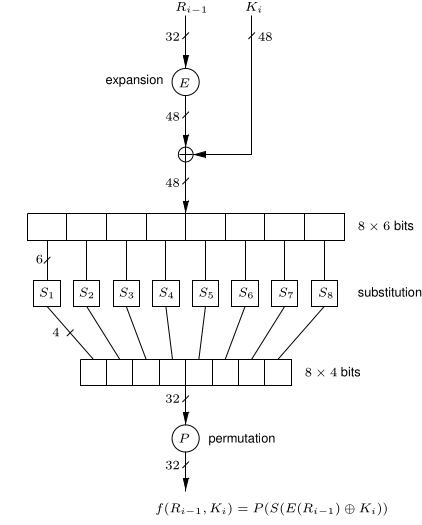
\includegraphics[scale=0.40]{Fonction_F.png}\end{center}
			\begin{center}\title{Schéma de la fonction F}\end{center}
			on obtient donc la formule suivant :
			\begin{center}$L_{16}'\oplus L_{16} = P(S(E(R_{15}')\oplus K_{16}))\oplus P(S(E(R_{15})\oplus K_{16})) $\end{center}
			
			De cette formule on peut enlever la permutation P car on connais l'emplacement des bits permuté et la permutaion P est linéaire.\\
			on a donc :
			\begin{center}$P^{-1}(L_{16}'\oplus L_{16}) =P^{-1}( P(S(E(R_{15}')\oplus K_{16}))\oplus P(S(E(R_{15})\oplus K_{16}))) $\end{center}
			\begin{center}$P^{-1}(L_{16}'\oplus L_{16}) =S(E(R_{15}')\oplus K_{16})\oplus S(E(R_{15})\oplus K_{16}) $\end{center}
			
			A ce stade on ne peut pas réduire plus cette formule car S est non linéaire donc je ne peux pas l'enlever comme j'ai fait avec la permutaion P.\\
			On va nommer deux variable $\alpha = E(R_{15})\oplus K_{16}$ et $\alpha' = E(R_{15}')\oplus K_{16}$.
			Par force brute on va déterminer tous les $\alpha'$ passant dans la sbox nous donnant les même bits de sorti avant permutaion. Cela représente une force brute sur $2^{6}$valeurs a tester.On effectuera cette tache pour chaque chiffré fauté en notre possession.\\
			Je vais étendre les $\alpha'$ obtenu jusqu'a 48bits pour pouvoir effectuer les calculs suivant tout en gardant l'emplacement de alpha parmis les 48bits rajouter.\\
			$R_{15}'$ est connu ($R_{16}'=R_{15}'$) donc je vais calculer l'expansion de $R_{15}'$ puis effectuer un xor entre cette expansion et les $\alpha'$ déterminer précédement. De faire ce calcul me permettra d'avoir 6 bit de la clef $K_{16}$ cependant j'aurai plusieurs candidats (noté $\gamma$) car j'ai plusieurs $\alpha'$.\\
			Dans un premier temps pour déterminer le bon candidat je vais calculer $\alpha$ avec comme clé un $\gamma$ a l'emplacement de la sbox touché par la faute ce qui nous donnera une clef de 48 bits.j'effectuerai cette opération autant de fois qu'il y a de $\gamma$.\\
			Dans un second temps, je passerai le résultat de $\alpha$ dans les sbox puis je vérifie que le résultat obtenu est le bon avant permuation. Si il est bon alors cela veut dire que j'ai trouvé les 6 bon bits de clef ($\gamma$) sinon je continue jusqu'a trouver le bon $\gamma$ me donnant la bonne sortie avant permuation.\\
			
			Exemple: la faute est situé au 30ème bit.\\
			
			on a donc :\\
			$S(E(R_{15})\oplus K_{16}$ = 01 ..... 1010 1110\\
			$E(R_{15}')$ = 10 ..... 1001 0110\\
			$\alpha_1'$= 00 ..... 0010 0111\\
			$\alpha_2'$= 00 ..... 0001 0100\\
			$\gamma_1=E(R_{15}')\oplus \alpha_1'$= 10 ..... 1011 0001\\
			$\gamma_2=E(R_{15}')\oplus \alpha_2'$= 10 ..... 1000 0010\\
			$\alpha_{\gamma_1}$= 01 ..... 1000 0101 , $\alpha_{\gamma_1}$ n'est pas le bon candidat car les 4 derniers bits sont différent de celui de $S(E(R_{15})\oplus K_{16}$.\\
			$\alpha_{\gamma_2}$= 00 ..... 0110 1110 , $\alpha_{\gamma_2}$ les 4 derniers bit sont équivalent à $S(E(R_{15})\oplus K_{16}$ donc les bit de 31 à 28 sont égaux a ceux de $\gamma_2$.\\
			
			Pour finir après avoir appliquer l'attaque décrite un peu plus haut j'obtiens la clef suivante: B1A6E1869A35
		\chapter{Retrouver la clef complète du DES}
			Pour retrouver 48bits des 56bits de la clef j'effectue le cadencement de clef a l'inverse de comment il est décrit.
			Une fois ces 48 bits déterminer, certains bits n'on pas de valeurs donc pour retrouver ces derniers 8 bits on va les faire varier en effectuant une force brute de $2^{8}$ valeurs. A chaque valeur on effectue le DES avec la nouvelle clef, tant que nous obtenons pas le bon chiffré en sorti on continue de faire varier les 8bits manquants. Une fois le bon chiffrer en sorti, la bonne clef de 56 bits a été trouvé.\\
			
			On obtient donc comme clef : E65875255B64BA40
		
		\chapter{Fautes sur les tours précédents}
			\section{attaque sur le 14ème tour}
			\section{attaque sur le 13ème tour}
			\section{généralisation sur le nième tour}
		
		\chapter{Contre-mesures}
			\section{Doublé le calcul du DES}
				Une solution assez simple qui nous vient en tête est de calculé deux/plusieurs fois l'algorithme du DES pour le même message puis véfirier si les résultats obtenu a la fin est
				identique.
				Si les résultats sont identique alors il n'y a pas eu d'injection de faute, sinon une faute a été introduite on ne renvoie rien.
				Cependant cette méthode est partiellement efficace car on peut partir du principe que l'attaquant a plusieurs outils similaires pour faire la fautes au même endroit a chaque fois et 
				donc que l'injection de faute soit un succès. 
				Il faudrait donc calculer n+1 fois le DES (n étant le nombre d'outils qu'a l'attaquant) pour espérer s'en protéger ce qui donnerai une compléxité très grande. 
				De plus si on voulais mettre cette solution dans une carte a puce on serait très vite limité au nombre de fois que l'ont puisse calculer le DES.
				La compléxité de cette solution serait de l'ordre K$\times$O(DES), K étant le nombre de fois que l'ont calcul le DES.
			
			\section{Diffusion de l'erreur}
				Une autre solution que j'ai discuté avec mon chargé de td est la diffusion de l'erreur. Plus précisément, le but est de propagé l'erreur a tous les bits, plusieurs fois de manières non linéaire pour que le chiffré obtenu par l'attaquant ne puisse lui donner aucune information sur la clef ou tout autre élément utile a l'attaquant.
				Cependant dans les fait cette solution n'a pas encore été réalisé pour le DES ou autre chiffrement du même type que le DES. Il y a un problème majeur avec cette méthode il faut déjà détecter la faute ce qui n'est pas trop compliqué en soit mais de cette détection découle le fait d'appliquer ou non la diffusion de la faute. A énoncé verbalement c'est simple mais dans les faits aucun modèle ou solution concrète n'a été décrite a ce jour dans la littérature Cryptographique.
		
		\chapter{Annexe}


		
\end{document}
